\documentclass{article}

\usepackage[dvipsnames]{xcolor}
\usepackage{ctex}
\usepackage{graphicx}
\usepackage[unicode]{hyperref}
\usepackage{cite}
\usepackage{indentfirst}
\usepackage{listings}
\usepackage{geometry}
\usepackage{amsmath}

\geometry{a4paper, left=2cm, right=2cm, top=1cm, bottom=1.5cm}

% \lstset{
%   language=C++,
%   basicstyle=\fontsize{8}{5}\ttfamily, % 设置代码字体大小为 12pt
%   breaklines=true, % 自动换行
%   numbers=left,
%   showstringspaces = false
% }

%%%%%% 设置字号 %%%%%% 
\newcommand{\chuhao}{\fontsize{nn42pt}{\baselineskip}\selectfont}
\newcommand{\xiaochuhao}{\fontsize{36pt}{\baselineskip}\selectfont}
\newcommand{\yihao}{\fontsize{28pt}{\baselineskip}\selectfont}
\newcommand{\erhao}{\fontsize{21pt}{\baselineskip}\selectfont}
\newcommand{\xiaoerhao}{\fontsize{18pt}{\baselineskip}\selectfont}
\newcommand{\sanhao}{\fontsize{15.75pt}{\baselineskip}\selectfont}
\newcommand{\sihao}{\fontsize{14pt}{\baselineskip}\selectfont}
\newcommand{\xiaosihao}{\fontsize{12pt}{\baselineskip}\selectfont}
\newcommand{\wuhao}{\fontsize{10.5pt}{\baselineskip}\selectfont}
\newcommand{\xiaowuhao}{\fontsize{9pt}{\baselineskip}\selectfont}
\newcommand{\liuhao}{\fontsize{7.875pt}{\baselineskip}\selectfont}
\newcommand{\qihao}{\fontsize{5.25pt}{\baselineskip}\selectfont}

% %%%% 设置 section 属性 %%%%
% \makeatletter
% \renewcommand\section{\@startsection{section}{1}{\z@}%
% {-1.5ex \@plus -.5ex \@minus -.2ex}%
% {.5ex \@plus .1ex}%
% {\normalfont\sihao\CJKfamily{hei}}}
% \makeatother

 %%%% 设置 subsection 属性 %%%%
% \makeatletter
% \renewcommand\subsection{\@startsection{subsection}{1}{\z@}%
% % {-1.25ex \@plus -.5ex \@minus -.2ex}%
% % {-1ex \@plus -.5ex \@minus -.2ex}%
% {-1ex \@plus -.3ex \@minus -.1ex}%
% {.4ex \@plus .1ex}%
% {\normalfont\xiaosihao\CJKfamily{hei}}}
% \makeatother

% %%%% 设置 subsubsection 属性 %%%%
% \makeatletter
% \renewcommand\subsubsection{\@startsection{subsubsection}{1}{\z@}%
% {-1ex \@plus -.5ex \@minus -.2ex}%
% {.3ex \@plus .1ex}%
% {\normalfont\xiaosihao\CJKfamily{hei}}}
% \makeatother

%%%% 段落首行缩进两个字 %%%%
\makeatletter
\let\@afterindentfalse\@afterindenttrue
\@afterindenttrue
\makeatother
% \setlength{\parindent}{2em}  %中文缩进两个汉字位

%%%% 下面的命令重定义页面边距,使其符合中文刊物习惯 %%%%
% \addtolength{\topmargin}{-54pt}
% \setlength{\oddsidemargin}{0.63cm}  % 3.17cm - 1 inch
% \setlength{\evensidemargin}{\oddsidemargin}
% \setlength{\textwidth}{14.66cm}
% \setlength{\textheight}{24.00cm}    % 24.62

%%%% 下面的命令设置行间距与段落间距 %%%%
\linespread{1.0}
% \setlength{\parskip}{1ex}
\setlength{\parskip}{0.5\baselineskip}

% 在导言区进行样式设置
\lstset{
    language=C++, % 设置语言
 	basicstyle=\ttfamily, % 设置字体族
 	breaklines=true, % 自动换行
 	keywordstyle=\bfseries\color{NavyBlue}, % 设置关键字为粗体,颜色为 NavyBlue
 	morekeywords={PressureSensor, Button, Oled}, % 设置更多的关键字,用逗号分隔
 	emph={self}, % 指定强调词,如果有多个,用逗号隔开
    emphstyle=\bfseries\color{Rhodamine}, % 强调词样式设置
    commentstyle=\itshape\color{black!50!white}, % 设置注释样式,斜体,浅灰色
    stringstyle=\bfseries\color{PineGreen!90!black}, % 设置字符串样式
    columns=flexible,
    numbers=left, % 显示行号在左边
    numbersep=2em, % 设置行号的具体位置
    numberstyle=\footnotesize, % 缩小行号
    % frame=single, % 边框
	tabsize = 4,  %行缩进
    framesep=1em % 设置代码与边框的距离
}

%%%% 正文开始 %%%%
\begin{document}	
		%%%% 定理类环境的定义 %%%%
\newtheorem{example}{例}             % 整体编号
\newtheorem{algorithm}{算法}
\newtheorem{theorem}{定理}[section]  % 按 section 编号
\newtheorem{definition}{定义}
\newtheorem{axiom}{公理}
\newtheorem{property}{性质}
\newtheorem{proposition}{命题}
\newtheorem{lemma}{引理}
\newtheorem{corollary}{推论}
\newtheorem{remark}{注解}
\newtheorem{condition}{条件}
\newtheorem{conclusion}{结论}
\newtheorem{assumption}{假设}

		%%%% 重定义 %%%%
\renewcommand{\contentsname}{目录}  % 将Contents改为目录
\renewcommand{\abstractname}{摘要}  % 将Abstract改为摘要
\renewcommand{\refname}{参考文献}   % 将References改为参考文献
\renewcommand{\indexname}{索引}
\renewcommand{\figurename}{图}
\renewcommand{\tablename}{表}
\renewcommand{\appendixname}{附录}
\renewcommand{\algorithm}{算法}	

		%%% 定义标题格式,包括title,author,affiliation,email等 %%%%
\title{智能仓储系统的开发研究}
% \author{XXX\footnote{电子邮件: XXXXXXXXXXXX@zjut.edu.cn 学号: XXXXXXXXXXXX}\\[2ex]
% \xiaosihao 浙江工业大学\\[2ex]}
\author{\xiaosihao 先进计算与机器人研究所}
%\date{}
		
		%%%% 以下部分是正文 %%%%  
\maketitle
		
\tableofcontents
\newpage

\section{第五章: 射频识别技术(RFID-RC522)}
在上一章中, 我们是直接给的物品种类以及单个物品质量的信息。实际上这是从RC522读卡器上的卡读到的。首先来认识RC522模块,
\begin{figure}[h]
	\centering
	\begin{minipage}{.45\textwidth}
		\centering
		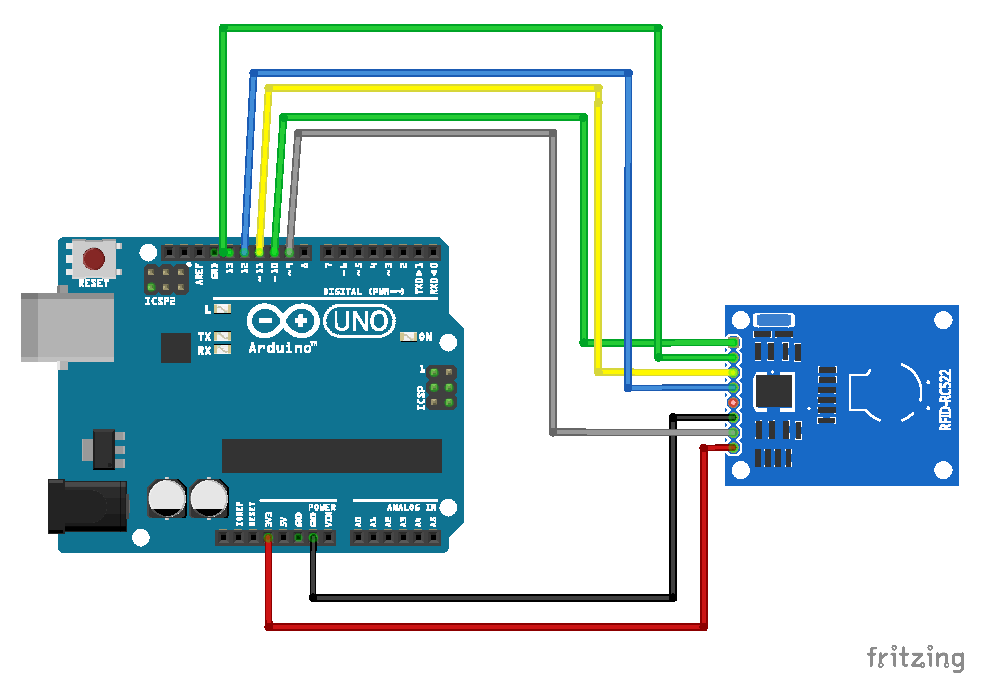
\includegraphics[width=\linewidth]{../Picture/RFID_RC522.pdf}
		\caption{RC522硬件连接}
		\label{fig:RC522硬件连接}
	\end{minipage}%
	\hfill
	\begin{minipage}{.45\textwidth}
		\centering
		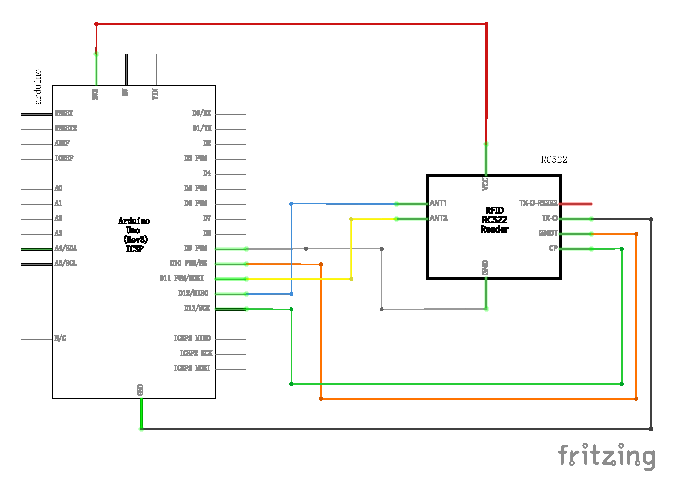
\includegraphics[width=\linewidth]{../Picture/RFID_RC522_line.pdf}
		\caption{RC522连接示意图}
		\label{fig:RC522连接示意图}
	\end{minipage}
\end{figure}

RC522模块共有8个与外界连接的引脚,与arduino的连接如图所示:

\begin{itemize}
	\item VCC为模块供电, 连接到Arduino的3.3V输出。;
	\item RST是复位和掉电的输入。当该引脚变为低电平时,关闭所有内部电流吸收器,包括振荡器,并且输入引脚与外界断开连接。在上升沿,模块被重置;
	\item GND是接地引脚,连接到Arduino的GND引脚;
	\item IRQ是一个中断引脚,可在RFID标签进入附近时向微控制器发出警报;
	\item 当使用SPI接线时, MISO上的数据从从机输出到主机;
	\item 当使用SPI接线时, MOSI上的数据从主机输出到从机;
	\item SCK是串行时钟信号, 由主机产生发送给从机;
	\item ss上信号由主机发送, 以控制与哪个从机通信, 通常是低电平有效信号。
\end{itemize}

在MFRC522模块上只有两个引脚RST和SS可以自己定义,这里将其定义为引脚9和引脚10(除了引脚11, 引脚12, 引脚13外的任意空闲数字引脚皆可, 引脚11,12,13
已经与RC522的引脚MOSI,MISO,SPI连接。将其定义为引脚9和引脚10是常见布局)。

\subsection{RC522类的声明}
RC522类就对应了整个RC522模块的功能。
\begin{lstlisting}
class RC522{
private:
  int RST_PIN, SS_PIN;
  MFRC522 mfrc522;                                           

public:
  char Type_Name[3];  
  long Single_Weight;
  long Shell_Weight;

  RC522();
  void initialize(int p1, int p2);
  byte read();
  bool write();
}	
\end{lstlisting}

\begin{itemize}
	\item 私有变量: RST\_PIN, SS\_PIN分别是与RC522的RST,SS连接的arduino引脚;
	\item 公共变量: Type\_Name, Single\_Weight, Shell\_Weight是储存从读卡器中读到的物品种类, 单个物品质量, 每一层物品质量;
\end{itemize}

默认构造函数:
\begin{lstlisting}
RC522::RC522(){};	
\end{lstlisting}

初始化函数用于引脚的赋值, 初始化SPI通信, 初始化MFRC522类。
\begin{lstlisting}
void RC522::initialize(int p1, int p2){
  RST_PIN=p1;
  SS_PIN=p2;
  SPI.begin();
  mfrc522 = MFRC522(SS_PIN, RST_PIN);                                           
  mfrc522.PCD_Init();  
};	
\end{lstlisting}


\subsection{读卡模式}
将下述代码烧录运行,就做好了读卡准备。
\begin{lstlisting}
byte RC522::read(){
  // init the read state
  byte read_state = 0;
  //default key 
  MFRC522::MIFARE_Key key;
  for (byte i = 0; i < 6; ++i) key.keyByte[i] = 0xFF;
  //some variables we need
  byte block;
  byte len;
  MFRC522::StatusCode status;
  //-------------------------------------------
  // Reset the loop if no new card present on the sensor/reader. This saves the entire process when idle.
  if ( ! mfrc522.PICC_IsNewCardPresent()) {
    return read_state;
  }
  // Select one of the cards
  if ( ! mfrc522.PICC_ReadCardSerial()) {
    return read_state ;
  }
  // read one card
  read_state = 1;
  Serial.println(F("**Card Detected:**"));
  //-------------------------------------------
  // mfrc522.PICC_DumpDetailsToSerial(&(mfrc522.uid)); //dump some details about the card
  // mfrc522.PICC_DumpToSerial(&(mfrc522.uid));      //uncomment this to see all blocks in hex
  //-------------------------------------------

  byte buffer1[18];
  block = 1;
  len = 18;
  //------------------------------------------- GET TYPE NAME
  status = mfrc522.PCD_Authenticate(MFRC522::PICC_CMD_MF_AUTH_KEY_A, block, &key, &(mfrc522.uid)); //line 834 of MFRC522.cpp file
  if (status != MFRC522::STATUS_OK) {
    Serial.print(F("Authentication failed: "));
    Serial.println(mfrc522.GetStatusCodeName(status));
    return read_state;
  }
  status = mfrc522.MIFARE_Read(block, buffer1, &len);
  if (status != MFRC522::STATUS_OK) {
    Serial.print(F("Reading failed: "));
    Serial.println(mfrc522.GetStatusCodeName(status));
    return read_state;
  }
  //PRINT TYPE NAME
  Type_Name[0] = buffer1[0];
  Type_Name[1] = buffer1[1];
  long singleweight = 0;
  for (uint8_t i = 2; i < 6; ++i)
  {
    singleweight = singleweight*10 + (buffer1[i]-48);
  }
  Single_Weight = singleweight;
  Serial.print(F("Type Name: "));
  Serial.println(Type_Name);
  Serial.print(F("Type Single Weight: "));
  Serial.println(Single_Weight);
  //---------------------------------------- GET WEIGHT

  byte buffer2[18];
  block = 4;
  status = mfrc522.PCD_Authenticate(MFRC522::PICC_CMD_MF_AUTH_KEY_A, block, &key, &(mfrc522.uid)); //line 834
  if (status != MFRC522::STATUS_OK) {
    Serial.print(F("Authentication failed: "));
    Serial.println(mfrc522.GetStatusCodeName(status));
    return read_state;
  }
  status = mfrc522.MIFARE_Read(block, buffer2, &len);
  if (status != MFRC522::STATUS_OK) {
    Serial.print(F("Reading failed: "));
    Serial.println(mfrc522.GetStatusCodeName(status));
    return read_state;
  }
  //PRINT WEIGHT
  int shellweight = 0;
  for (uint8_t i = 1; i < 16; ++i) {
    // Serial.write(buffer2[i] );
    // Serial.println();
    // Serial.println(buffer2[i]);
    if(buffer2[i] == 32) break;
    shellweight =   shellweight*10 + (buffer2[i]-48);
  }
  Shell_Weight = shellweight;
  Serial.print(F("Shell Weight: "));
  Serial.println(Shell_Weight);
  //----------------------------------------
  Serial.println(F("**End Reading**\n"));
  read_state = 2;
  mfrc522.PICC_HaltA();
  mfrc522.PCD_StopCrypto1();
  return read_state;
}
\end{lstlisting}

\subsection{写卡模式}
将下述代码烧录运行,就做好了写卡准备。写卡时会在串口提示输入两次字符串, 每次都是以\#结尾。第一次是输入物品种类以及单个物品质量, 例如'AA0010\#'表示
物品种类是'AA',单个物品质量是10g;第二次是输入外壳质量, 例如'0\#'表示外壳质量是0。
\begin{lstlisting}
bool RC522::write(){
  //初始化读卡状态
  //未读到卡为0,读到卡为1
  bool write_state = 0;
  //创建访问密钥,用于验证并访问 MIFARE Classic RFID标签
  //这里用默认卡密钥
  MFRC522::MIFARE_Key key;
  for (byte i = 0; i < 6; i++) key.keyByte[i] = 0xFF;

  //block为卡的不同区域编号
  //len3为读到的字节数
  //status为判断对卡操作是否成功完成的状态变量
  byte block;
  byte len3;
  MFRC522::StatusCode status;

  // 如果传感器/读卡器上没有新卡,则复位循环。这可以在空闲时保存整个进程。
  if ( ! mfrc522.PICC_IsNewCardPresent()) {
    return write_state;
  }

  // 选择一张卡片进行读取
  if ( ! mfrc522.PICC_ReadCardSerial()) {
    return write_state;
  }

  Serial.println(F("**Card Detected:**"));
  // 成功读取到卡片,将读卡状态设为1
  write_state = 1;
  
  //打印UID编号
  Serial.print(F("Card UID:"));    
  for (byte i = 0; i < mfrc522.uid.size; i++) {
    Serial.print(mfrc522.uid.uidByte[i] < 0x10 ? " 0" : " ");
    Serial.print(mfrc522.uid.uidByte[i], HEX);
  }
  //打印PICC类型
  Serial.print(F(" PICC type: "));   
  MFRC522::PICC_Type piccType = mfrc522.PICC_GetType(mfrc522.uid.sak);
  Serial.println(mfrc522.PICC_GetTypeName(piccType));  

  byte buffer3[34];
  //等待20秒从串口输入
  Serial.setTimeout(20000L) ;     
  // 提示:输入类型名称
  Serial.println(F("Type name, ending with #"));
  //从串口读入类型名称到buffer3,len为写入字节长度
  len3 = Serial.readBytesUntil('#', (char *) buffer3, 30) ; 
  // 将未满字节用空格填补
  for (byte i = len3; i < 30; i++) buffer3[i] = ' ';     

  block = 1;
  //选择读取区域和密钥进行身份验证,验证失败打印错误信息并提前终止
  status = mfrc522.PCD_Authenticate(MFRC522::PICC_CMD_MF_AUTH_KEY_A, block, &key, &(mfrc522.uid));
  if (status != MFRC522::STATUS_OK) {
    Serial.print(F("PCD_Authenticate() failed: "));
    Serial.println(mfrc522.GetStatusCodeName(status));
    return write_state;
  }
  else Serial.println(F("PCD_Authenticate() success: "));

  // 对前述验证成功的区域内的信息写入字节数组,写入失败打印错误信息并提前终止
  status = mfrc522.MIFARE_Write(block, buffer3, 16);
  if (status != MFRC522::STATUS_OK) {
    Serial.print(F("MIFARE_Write() failed: "));
    Serial.println(mfrc522.GetStatusCodeName(status));
    return write_state;
  }
  else Serial.println(F("MIFARE_Write() success: "));

  block = 2;
  //选择读取区域和密钥进行身份验证,验证失败打印错误信息并提前终止
  status = mfrc522.PCD_Authenticate(MFRC522::PICC_CMD_MF_AUTH_KEY_A, block, &key, &(mfrc522.uid));
  if (status != MFRC522::STATUS_OK) {
    Serial.print(F("PCD_Authenticate() failed: "));
    Serial.println(mfrc522.GetStatusCodeName(status));
    return write_state;
  }

  // 对前述验证成功的区域内的信息写入字节数组的地址,写入失败打印错误信息并提前终止
  status = mfrc522.MIFARE_Write(block, &buffer3[16], 16);
  if (status != MFRC522::STATUS_OK) {
    Serial.print(F("MIFARE_Write() failed: "));
    Serial.println(mfrc522.GetStatusCodeName(status));
    return write_state;
  }
  else Serial.println(F("MIFARE_Write() success: "));

  byte buffer4[34];
  byte len4;
  // Ask personal data: First name
  Serial.println(F("Type Weight, ending with #"));
  len4 = Serial.readBytesUntil('#', (char *) buffer4, 20) ; // read first name from serial
  for (byte i = len4; i < 20; i++) buffer4[i] = ' ';     // pad with spaces

  block = 4;
  //选择读取区域和密钥进行身份验证,验证失败打印错误信息并提前终止
  status = mfrc522.PCD_Authenticate(MFRC522::PICC_CMD_MF_AUTH_KEY_A, block, &key, &(mfrc522.uid));
  if (status != MFRC522::STATUS_OK) {
    Serial.print(F("PCD_Authenticate() failed: "));
    Serial.println(mfrc522.GetStatusCodeName(status));
    return write_state;
  }

  // 对前述验证成功的区域内的信息写入字节数组,写入失败打印错误信息并提前终止
  status = mfrc522.MIFARE_Write(block, buffer4, 16);
  if (status != MFRC522::STATUS_OK) {
    Serial.print(F("MIFARE_Write() failed: "));
    Serial.println(mfrc522.GetStatusCodeName(status));
    return write_state;
  }
  else Serial.println(F("MIFARE_Write() success: "));

  block = 5;
  //选择读取区域和密钥进行身份验证,验证失败打印错误信息并提前终止
  status = mfrc522.PCD_Authenticate(MFRC522::PICC_CMD_MF_AUTH_KEY_A, block, &key, &(mfrc522.uid));
  if (status != MFRC522::STATUS_OK) {
    Serial.print(F("PCD_Authenticate() failed: "));
    Serial.println(mfrc522.GetStatusCodeName(status));
    return write_state;
  }

  // 对前述验证成功的区域内的信息写入字节数组的地址,写入失败打印错误信息并提前终止
  status = mfrc522.MIFARE_Write(block, &buffer4[16], 16);
  if (status != MFRC522::STATUS_OK) {
    Serial.print(F("MIFARE_Write() failed: "));
    Serial.println(mfrc522.GetStatusCodeName(status));
    return write_state;
  }
  else Serial.println(F("MIFARE_Write() success: "));
  delay(1000); 

  //--------------成功完成读取----------------
  Serial.println(F("\n**End Reading**\n"));
  //停止响应当前正在运行的命令。
    //将 RFID 卡片置于休眠状态,以便进行下一个命令的执行。
  mfrc522.PICC_HaltA();
  //停止当前正在进行的加密。如果 RFID 模块正在与 RFID 卡片进行加密通信,
  //则此代码将停止加密,并将模块置于初始状态,以便进行下一个操作。
  mfrc522.PCD_StopCrypto1();
  //返回写卡状态
  return write_state;
}
\end{lstlisting}

\subsection{RC522.ino}
在上一章master.ino基础上, 加入了通过读卡获得rc522的Single\_Weight和Type\_Name。并通过rflag是否为1判断是读还是写。目前有一点不妥的是, 当没有读到卡时, 在switch语句中
会一直在while中循环直到读到卡。也就是说即使物品总质量发生变化, 也只有在重新放卡后才能发送消息到上位机, 要不然出不了while循环语句。
\begin{lstlisting}
  #include "master.h"
  #include "transform.h"
  #include "Surface.h"
  #include "Calibrate.h"
  #include "Oled.h"
  #include "RC522.h"
  
  master m1;
  Surface YL_Surface;
  Calibrate YL_Calibrated;
  transform tf;
  Oled oled;
  RC522 rc522;
  
  long numbefore=0, numnow=1;
  char te[3];
  unsigned long Sweight;
  bool rflag=1;  //1 ---> read; 0 ---> write
  
  void setup() {
    Serial.begin(9600);
    m1.initialize(8);    //8needschanged
    YL_Calibrated.setpin_SCKDT(4, 5);
    YL_Calibrated.set_range(20);
    YL_Calibrated.kb_Initialize();
    oled.initialize();  
    rc522.initialize(9,10);
  }
  
  void loop() {
    switch(rflag){
      case 0: 
        while(1) {
          bool state = rc522.write();
          if(state==1)
            break;
        }   
        rflag=1;
        break;
      case 1:
        while(1) {
          bool state = rc522.read();
          if(state==1)
            break;
        }
        break;
    }
    for (int i=0; i<sizeof(rc522.Type_Name);i++) te[i]=rc522.Type_Name[i];
    Sweight=rc522.Single_Weight;
  
    numbefore = numnow;
    unsigned long CalibratedWeight = YL_Calibrated.Output_CalibratedWeight(YL_Surface.Get_Surface());
    numnow = ceil(CalibratedWeight/Sweight);
  
    bool flag= (numbefore==numnow?0:1);
    if(flag){
    tf.initialize(te, m1.address, numnow, CalibratedWeight);
    tf.pack();
    digitalWrite(3,HIGH);
    m1.send(9, tf.Transmission_Information);
    Serial.println(tf.Transmission_Information);
    oled.showIIC(te, numnow);
    digitalWrite(3,LOW);
    }
  
    delay(3000);
  }  
\end{lstlisting}

\end{document} 

